\chapwithtoc{Introduction}
\label{intro}

\secwithtoc{Proteins and domains}
\label{intro:prodoms}

  Proteins are amino acid chains, polypeptides, that serve a variety of functions within
  living cells, including structural support and movement, interactions with cell's
  environment, and biochemical reaction catalysis~\cite{alberts2018molecular}.
  To function properly, proteins have to fold into their native conformation, and as
  demonstrated by \citet{anfinsen1961kinetics} on bovine pancreatic ribonuclease, the
  information for correct folding is contained in the amino acid sequence itself.

  Different sequences fold into different three-dimensional conformations.
  Certain local regions form secondary structures, such as $\alpha$-helices and
  $\beta$-sheets, and these locally ordered regions associate to form the whole protein,
  or in the case of some larger proteins, to form folding units~\cite{levitt1975computer}.
  If the folding units would be stable, given that the polypeptide chain connecting them
  to the rest of the protein molecule were to be cleaved, these subassemblies can be
  referred to as \emph{domains}~\cite{goldberg1969tertiary, levitt1975computer}.
  Nevertheless, today's definition requires that these subassemblies also conceivably
  function in isolation, and members of the same \emph{domain family} tend to possess an
  ancient evolutionary relationship and often a similar
  function~\cite{ponting2002natural}.

  Many bioinformatics tools are available online to perform domain identification within
  a protein sequence.
  The \emph{SCOP} database organizes proteins of known three-dimensional structures
  according to their evolutionary and structural relationship~\cite{murzin1995scop}.
  It classifies non-redundant protein domains and defines them on two main levels of SCOP
  classification, family and superfamily.
  The designation of proteins in SCOP has been constructed mainly
  manually~\cite{andreeva2020scop}.

  Other tools tend to implement semimanual approaches, typically including a
  \emph{profile hidden Markov Model} (HMM), a powerful probabilistic method describing the
  sequence conservation in a family~\cite{krogh1994hidden, eddy1996hidden}.
  \emph{Pfam}~\cite{sonnhammer1997pfam} is such an example.
  Each protein family in Pfam database consists of a seed alignment forming the basis to
  build a HMM-based profile~\cite{el2019pfam} by engaging the HMMER
  software~\cite{finn2010pfam, finn2011hmmer}.
  Another protein structure classification database using HMMs to scan protein sequences
  against it is called \emph{CATH}~\cite{dawson2017cath}.
  CATH clusters proteins on four main levels, class (C), architecture (A), topology (T),
  and homologous superfamily (H)~\cite{orengo1997cath}.
  CATH, Pfam, and many more, are then integrated in a general resource for protein
  families, domains, and functional sites, called InterPro~\cite{finn2017interpro}.
  The authors aim to create a non-redundant characterization, and the software package
  InterProScan provides an interface to functionally classify novel nucleotide or protein
  sequences~\cite{zdobnov2001interproscan}.
  By uniting member databases, InterPro exploits their individual strengths, thus
  significantly contributing in the troublesome effort of automatic
  annotation~\cite{apweiler2000interpro}.

  \citet{chothia1992one} predicted that there is a limited number of protein families
  nature uses in evolution.
  Later, \citet{wolf2000estimating} estimated the sum to be between 4,000 and 7,000, and
  the Pfam database seems to confirm this calculation, as it records 6,248 family entries
  in release 32.0~\cite{el2019pfam}.

\secwithtoc{Protein kinase family}
\label{intro:pkinase}

  \begin{figure}
    \centering
    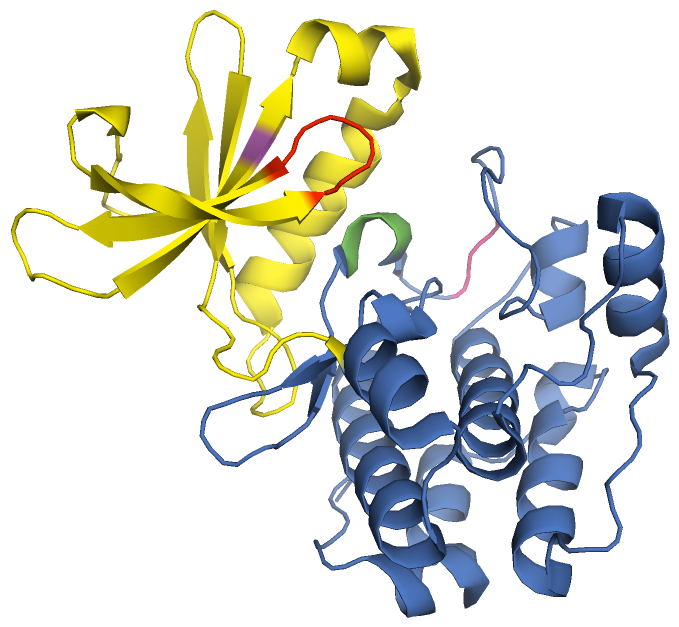
\includegraphics[width=0.8\linewidth]{img/aurora.png}
    \caption{The bilobal structure of the protein kinase domain from the Aurora A protein
    kinase.
    Structure downloaded from the PDBe, entry code 4dee~\cite{lawrence2012development},
    visualized with the PyMOL Molecular Graphics System~\cite{PyMOL}.
    Yellow: The small lobe.
    Blue: The large lobe.
    Red: Gly-X-Gly-X-X-Gly motif.
    Magenta: The invariant lysine.
    Green: DFG motif.
    Pink: APE motif.
    }
    \label{fig:aurora}
  \end{figure}

  An example of a protein family is the \emph{protein kinase family}, labeled as
  \texttt{PF00069} is the Pfam database.
  It is large and diverse~\cite{hanks1988protein, hunter19911}, and generally, protein
  kinases are involved in most of the signal transduction in eukaryotic cells.
  They control a variety of cellular processes, among other things metabolism, cell cycle
  progression, differentiation, transcription, cell movement, communication, and
  apoptosis~\cite{kemp2003amp, matsuoka1998linkage, johnson1994sequential,
  vermeulen2003transcriptional, chen1994cell, warn1998regulation, cross2000serine}.
  As protein kinases function as a responsive regulatory system, it is not surprising that
  their turnover rate is rather fast, with a half-life averaging less than an
  hour~\cite{hunter1982phosphotyrosine}.
  And because kinase activity at the wrong place or at the wrong time can lead to
  unfavorable cell transformation and cancer~\cite{koivunen2006protein,
  caretta2011protein}, they are a fascinating subject in molecular biology and
  bioinformatics.

  The conformational space of protein kinase domains is conserved~\cite{ung2018redefining}
  with common structural features specific to the protein kinase
  family~\cite{taylor1994three}.
  The enzyme structure is bilobal.
  The smaller lobe on the N-terminus is composed of a five-stranded antiparallel
  $\beta$-sheet and one $\alpha$-helix~\cite{knighton1991crystal} called $\alpha$C, which
  takes part in the stabilization of the active
  conformation~\cite{mobitz2015abc, huse2002conformational}.
  The broadly helical larger lobe associated with the C-terminus adds up to have seven
  $\alpha$-helices and one antiparallel $\beta$-sheet placed on the surface of the cleft
  between the two lobes, where the catalytic site is
  located~\cite{knighton1991crystal, taylor1994three, azam2008activation}.
  Twelve major subdomains can be further recognized throughout the protein kinase
  family~\cite{hanks1988protein, hanks19912, hanks1995eukaryotic}.

  Multiple sequence alignments of domains from the protein kinase family uncover many
  highly conserved residues and motifs, some of which are strictly required for the kinase
  activity.
  The nucleotide binding consensus sequence Gly-X-Gly-X-X-Gly is found in subdomain I and
  contains the first, second, and third essential glycine.
  Any side chain at glycines' positions would interfere with the incoming ATP (or GTP).
  The whole motif turns sharply around the nucleotide, with the first essential glycine
  being in contact with ribose, while the second provides space for the pyrophosphate
  group~\cite{wierenga1983predicted, hanks1988protein}.
  The $\beta$-phosphate moiety's oxygens are hydrogen bonded with the backbone amides of
  residues around the third fundamental glycine, and side chains surrounding this motif
  contribute to the hydrophobic pocket for the adenine ring of
  ATP~\cite{hanks1995eukaryotic}.
  GTP can be utilized as well, however, ATP will always have a lower Michaelis constant
  $\mathrm{K_{m}}$~\cite{hunter1985protein}.
  Regardless which, the phosphate donor is bound as a complex together with a divalent
  cation, with $\mathrm{Mn^{2+}}$ usually preferred over $\mathrm{Mg^{2+}}$ and
  others~\cite{witte1980abelson, richert1979characterization, wong1984purification}.

  An invariant lysine in subdomain II corresponding to PKA-C$\alpha$ Lys72 is thought to
  be the best characterized catalytic domain residue~\cite{hanks1988protein}.
  It forms a salt bridge with the carboxyl group of the practically invariant glutamate in
  subdomain III, which stabilizes the interactions between the lysine and the $\alpha$-
  and $\beta$-phosphates of ATP~\cite{hanks1995eukaryotic}.
  As \citet{kamps1986neither} showed in their work on p60\textsuperscript{\textit{src}}
  tyrosine protein kinase, all substitutions of the lysine, including arginine and
  histidine, result in loss of protein kinase activity.

  Highly conserved triad Asp-Phe-Gly (DFG) can be found in subdomain VII.
  It is part of the so called activation loop and helps orient the $\gamma$-phosphate of
  the ATP for transfer~\cite{hanks1995eukaryotic}.
  The activation loop is centrally located and provides a platform for a peptide
  substrate by interacting with the
  $\alpha$C-helix~\cite{huse2002conformational, mobitz2015abc}.
  Autophosphorylation of three conserved tyrosines within the activation loop results in
  an active kinase state, unphosphorylated loop traverses through the cleft between
  the two lobes of the kinase domain, thus yielding both protein substrate and ATP binding
  sites inaccessible~\cite{hubbard1997crystal}.
  The recognition of peptide substrates in the active state is then mediated by the
  Ala-Pro-Glu (APE) motif located in subdomain VIII~\cite{hanks1995eukaryotic}.

  Many other hydrophobic residues that do not form any primary sequence motif, or any
  particular secondary structure, characterize active kinases, as they either stabilize
  the whole domain, or regulate its overall
  activity~\cite{kornev2006surface, kornev2010defining}.
  Especially one residue called the ``gatekeeper'' lying in the hinge region between the N
  and C lobes of the kinase domain has recently been of great interest in kinase inhibitor
  development.
  This gatekeeper residue guards a small hydrophobic cavity neighboring the ATP-binding
  site~\cite{noble2004protein} and it anchors kinase inhibitors bound in the ATP
  pocket~\cite{tong1997highly, azam2008activation}.
  The particular type of the gatekeeper residue is specific to each protein kinase domain
  and the size and shape of the side chain determines the cavity's druggability.
  Moreover, drug design is strongly affected by the adjacent DFG motif's conformation as
  well~\cite{zuccotto2010through}.

  Still, not all members of the protein kinase family possess the kinase enzymatic
  activity~\cite{zervas2002integrin, morrison2001ksr, kroiher2001deceiving}.
  Such seemingly inactive domains may have hypothetical noncatalytic functions, or do not
  require the conserved catalytic residues mentioned above and use a modified catalytic
  mechanism instead~\cite{manning2002protein}.
  However, as about two thirds of prokaryote proteins and aroung eighty percent of
  eukaryote proteins are multi-domain
  proteins~\cite{teichmann1998structural, gerstein1998representative}, kinase domains can
  primarily also modulate other catalytic regions.

\secwithtoc{Multi-domain proteins}
\label{intro:multi}

  With a limited number of domain families
  present~\cite{chothia1992one, wolf2000estimating}, creating new functions may be somehow
  difficult.
  Nature overcomes this obstacle by combining old building blocks instead of inventing new
  ones~\cite{apic2001insight}.
  \citet{muller2002structural} estimated that 98\% of the domains in the human proteome
  are duplicates, duplication is in fact one of the main sources for creation of new
  genes~\cite{lynch2000evolutionary}.
  Consequently, it is not surprising that the major molecular mechanism leading to
  multi-domain proteins and novel combination is non-homologous recombination, which is
  sometimes referred to as ``domain shuffling''~\cite{vogel2004structure}.

  Domains are not merged aimlessly, when creating multi-domain proteins.
  Domain combinations seen in nature can be discriminated from a random model of domain
  combination, as shown by \citet{apic2003multi}.
  Putting together specific superfamilies results in more specific functions for
  individual molecules, and proteins with the same domain arrangement tend to be
  evolutionarily and functionally
  related~\cite{hegyi2001annotation, bashton2002geometry, vogel2004structure}.
  The sequential order of protein families identified within a protein is called
  \emph{architecture}.

  The set of all architectures seems to be limited as well.
  A pattern is observed, where most domains tend to have only one or few
  combination partners in multi-domain proteins.
  Moreover, if a domain is found on the N-terminus of a multi-domain protein, other
  members of the same family are usually to be found on the N-terminus as well, and vice
  versa.
  The orientation and type of neighborhood varies only in few domain families, most of
  these are large and versatile~\cite{apic2001domain, apic2001insight}.

\subsecwithtoc{Non-domain regions}
\label{intro:linker}

  Domains within the same protein are connected by non-domain amino acid stretches.
  These can be long or short, often having a disordered structure, and considering the
  limited number of domains and architectures in nature, these \emph{linkers} introduce
  new possibilities for structural assemblies, and may regulate, or sometimes even take
  part in proteins' activity and stability~\cite{papaleo2016role}.
  Therefore, depending on a functionality given by a domain, its associated linker
  generally requires a certain amino acid sequence~\cite{gokhale2000role}.
  It has been shown by \citet{jakubec2018widespread} that residues in pairs of domains
  coevolve, and responses to mutations in residue pairs are also observed in non-domain
  regions~\cite{smock2010interdomain}, thus ensuring a suitable environment for the whole
  molecule.

  Linkers often serve as rigid spacers between two domains.
  These molecular rulers are mostly $\alpha$-helical, and they prevent unfavorable
  interactions between the neighboring
  modules~\cite{george2002analysis, wriggers2005control}.
  Mutations in such non-domain regions are not expected to affect the function of a
  protein in any way~\cite{bottema1991missense}, in different circumstances, however,
  alterations in the linker region can have effect on stability, proteolytic resistance,
  or solubility of single-chain proteins~\cite{robinson1998optimizing}.
  Especially, careful selection of residues around prolines is of utmost importance.
  Proline is the most common residue in linkers.
  Its stiff nature helps prevent ominous contacts of linkers and domains, as it can not
  participate comfortably in any standard secondary structure conformation due to its
  inability to hydrogen bond to other
  moieties~\cite{george2002analysis, wriggers2005control}.
  Other amino acids typical to linkers are glutamine, less specifically polar and charged
  amino acids, contrarily, residues with hydrophobic or aromatic side chains are more
  common in domains~\cite{brune2018proteome}.

  Nevertheless, many linkers are also soft and intrinsically distorted.
  The non-domain region of human immunoglobulin G1 exemplifies such flexible amino acid
  sequence~\cite{colman1976structure}.
  These often promote fundamental catalytic events in the overall function of proteins, as
  observed in the packaging of the tomato bushy stunt virus
  protein~\cite{winkler1977tomato}.
  Since soft linkers connecting domains are not merely flexible, but also allosterically
  regulated, it is no wonder that they are capable of facilitating protein folding and
  conformational changes of the whole molecule, as the amino acid sequences of linkers,
  and particularly of the residues in contact between linkers and adjoint domains,
  encode conformational states, through which signals
  travel~\cite{george2002analysis, ma2011dynamic}.
  Prototypes of such signals may be phosphorylation of a distant residue, or, for example,
  ATP binding.
  Otherwise flexible linker in Src kinases clamps SH2 and SH3 domains upon C-terminal
  tyrosine phosphorylation~\cite{young2001dynamic}, ATP binding on the other hand causes
  the immobilization of neck linkers of kinesins, which subsequently extend towards the
  plus end of a microtubule, thus giving kinesins their forward
  drive~\cite{rice1999structural, rosenfeld2001atp, khalil2008kinesin}.

  Both changes in linker length and composition can alter folding kinetics, function, and
  stability of proteins~\cite{van1997linker, robinson1998optimizing}, as demonstated in
  many studies.
  A dramatic increase of pI from 5.86 to 9.81 was observed after deletion of 40
  residues of a linker of mycobacteriophage D29 endolysin~\cite{pohane2015modulation},
  conformations of protein domains in cellulosomes are primarily influenced by the length
  of the linkers, as the stiffness of the linkers is negatively proportional to the linker
  length~\cite{rozycki2017length}, and in the kinesins mentioned above, the effectivity of
  kinesin runs is determined by the length of the neck linker~\cite{shastry2010neck}.
  Domain functions are predominantly affected by short linkers, notably those that
  are buried as well, contrarily, long linkers allow similar relative positions between
  domains with swapped sequential order to be achieved, hence not having so much impact
  on the overall protein activity~\cite{bashton2002geometry}.

  Other authors present examples, where amino acid composition is more relevant for
  the protein function compared to length.
  \citet{klement2015effect} concluded this after exploring the functionality of cytotoxic
  engineered antibody fragments.
  In further research, \citet{ikebe1998hinge} demonstrated the importance of selected
  residues in smooth muscle myosins with their actin translocating activity terminated
  upon deletion or substitution of these amino acids, and conserved linker sequence is
  crucial for the already discussed kinesins' microtubule-based motility as
  well~\cite{case2000role, hariharan2009insights}.

  Yet, it remains to be uncovered, \emph{how} the composition of non-domain regions
  affects the function of multi-domain proteins.
  For instance, even though not only the common structural elements of protein kinases are
  involved in their regulation, but for many kinases also by
  linkers~\cite{gogl2019disordered}, these non-core segments remarkably do not show any
  sequence similarity, and differ overall throughout the protein kinase
  family~\cite{taylor1994three}.
  This thesis aims to expose the relationship between the linkers' composition and protein
  activity and specificity.
  This will be done by analyzing sequences of two-domain proteins containing exactly
  one protein kinase domain, clustering the inter-domain stretches by computationally
  acquired physicochemical properties, and embedding unique \emph{Gene Ontology}
  (GO)~\cite{ashburner2000gene, gene2019gene} and \emph{Enzyme Commission number}
  (EC)~\cite{webb1992enzyme, jeske2019brenda} terms into defined linker groups.
